% vim:spell spelllang=sk
%\subsection{Image compression}
\section{Image compression}

%% {{{ zakladny nacrt kompresie
%\subsubsection{Základný náčrt kompresie údajov}
\subsection{Základný náčrt kompresie údajov}
Stratová (ale aj bezstratová) kompresia údajov je založená na
jednoduchých princípoch. Jej hlavné črty si môžeme popísať v~troch
krokoch
\begin{itemize}
\item Transformácia
\item Kvantizácia
\item Kompresia
\end{itemize}
Poďme sa bližšie zaoberať jednotlivými časťami.
Transformácia je bezstratová manipulácia s~údajmi. Transformáciou môže
byť identita, rozdelenie obrazu na farebné zložky, zmena RGB na CMYK 
a~pod. Hlavnou úlohou transformácie je akosi predpripraviť dáta na
ďalšie spracovanie, dostať ich do vhodnej podoby pre ďalšie kroky, ale
pritom vedieť stále vypočítať reverznú transformáciu. Krok
transformácie je zároveň krokom, kedy sa teoreticky
\footnote{V praxi môže dochádzať k chybám zo zaokrúhľovania}
nestráca žiadna informácia.

Nasleduje, druhý krok, samotný krok zodpovedný za stratu informácie
pri stratovej kompresii. Pri bezstratovej kompresii je samozrejme
vynechaný. Výstupom z~transformácie sú dáta. Tieto dáta môžeme
považovať za reálne resp. celé čísla. Ich problémom je veľká pamäť
potrebná na udržiavanie týchto informácii. Kvantizácia rieši tento
problém jednoducho inžiniersky - nejaké informácie vynecháme.
Spravidla sa to robí tak, že čísla sa vydelia kvantizačným faktorom 
a~zaokrúhlia nadol. Opačný proces ku kvantizácii môže len hádať pôvodné
čísla, preto je kvantizácia stratová. Je však na umení príslušného
spôsobu kvantizácie, aké to bude mať vizuálne následky. Ako vieme,
väčšina informácie skrytá v~digitálnych obrázkoch či zvukoch je
takpovediac nepotrebná. Človek nemá natoľko vyvinuté zmysly, aby ju
všetku videl/počul. Preto záleží len na šikovnosti, ktoré informácie
budú kvantizované viac a~ktoré menej. Samozrejme, snahou je najviac
kvantizovať informácie pre človeka skryté a~naopak, dôležité údaje
nekvantizovať vôbec. Tu si kvantizácia podáva ruku s~predchádzajúcou
transformáciou - čím lepšie transformácia oddelí dôležité od
nedôležitého, tým lepšie vieme kvantizovať.

Poslednou časťou je kompresia. Toto je čiste bezstratová kompresia,
ktorá sa snaží ešte z~kvantizovaných údajov vyžmýkať posledné voľné
bity a~tak zavŕšiť finálnu podobu.

Príkladom formátu, ktorý nemá transformáciu, nemá kompresiu ale má
kvantizáciu je napríklad BMP - kvantizuje každú farebnú zložku do 8
bitov. Formátom bez transformácie s kvantizáciou a kompresiou môže byť
napríklad TGA - prebieha v~ňom Run-length kompresia, ktorá vie dobre
komprimovať dlhé úseky rovnakej farby.
V~skutočnosti, najviac účinné formáty sú tie, ktoré používajú
sofistikovanú transformáciu. Príkladom je JPEG2000 využívajúci
waveletovú transformáciu či klasický formát JPEG. Práve pri ňom sa
teraz zastavíme a~bližšie si popíšeme jeho kroky.
%% }}}

%% {{{ farebna predpriprava
%\subsubsection{Jpeg - farebná predpríprava}
\subsection{Jpeg - farebná predpríprava}
Dátový formát jpeg je sofistikovaný formát využívajúci viaceré
poznatky z~vizuálneho vnímania obrazu.

V~počítači je bežná reprezentácia farieb v~takzvanom RGB móde, kde
farba pozostáva z~koordinátov v 3D priestore (Červená, Zelená, Modrá).
Hoci je tento spôsob veľmi intuitívny pre CRT monitory, nie je
perfektný pre kompresiu. Trojica farieb červená, zelená a~modrá totiž
nepopisuje spôsob vnímania ľudskou bytosťou rovnomerne. Formát JPEG
rieši tento problém zavedením nového farebného priestoru $(Y,Cb,Cr)$,
ktorý sa dá vypočítať nasledovne \footnote{Prevzaté z \cite{jfif}} 
(predpokladáme 8-bitové RGB hodnoty)
\begin{align*}
    Y &= 0.299 R + 0.587 G + 0.114 B \\
    Cb &= -0.1687R - 0.3313G + 0.5B + 128 \\
    Cr &= 0.5R - 0.4187 G - 0.0813B + 128
\end{align*}
Pričom spätná transformácia je
\begin{align*}
    R &= Y + 1.402 (Cr - 128) \\
    G &= Y - 0.34414 (Cb-128) - 0.71414 (Cr-128) \\
    B &= Y + 1.772 (Cb - 128)
\end{align*}
Nasleduje prvá kvantizácia nazývaná Chroma subsampling, 
kde sa zložky  $Cr, Cb$ redukujú na nižšie
rozlíženie. Ľudské oko je totiž omnoho menej citlivé na zmenu farby
ako na zmenu jasu. Pri kompresii si preto môžeme dovoliť zmenšiť
rozlíšenie s~akým je uchovaná farba.
Nepríjemným vedľajším dôsledkom môže byť "pretekanie" farebného
odtieňa na silno kontrastných hranách.
\begin{poznamka}
Viac o~subsamplingu sa čitateľ môže dozvedieť v 
\cite{subsampling}.
\nocite{wiki:chroma}
\end{poznamka}
%% }}}


%% {{{ DCT
%\subsection{Jpeg - kosínová transformácia}
\subsection{Jpeg - kosínová transformácia}

Po tejto úprave sa všetky tri vrstvy spracúvajú samostatne a~tým
istým spôsobom. Snahou je zredukovať ďalšiu nepotrebnú informáciu.
Práve tu sa ujíma vedenia Fourierova transformácie, presnejšie
povedané jej kamarátka diskrétna kosínová transformácia. Jej špeciálna
verzia pre JPEG sa od vzorca \ref{eq:dct_transform} 
líši normalizáciou a~špecializáciou na vstup veľkosti $8\cross8$.
\begin{equation}
   F(u,v) = \frac{1}{4} C(u) C(v) 
    \sum_{x=0}^7 \sum_{y=0}^7 f(x,y)
        \cos\frac{\pi(x+1/2) u }{8}
        \cos\frac{\pi(y+1/2) v }{8}
    \label{eq:dct_jpeg}
\end{equation}
Kde $C$ je definované ako
\begin{equation*}
    C(u) = \left\{
        \begin{array}{l l}
            \frac{1}{\sqrt{2}} & u=0 \\
            1 & u\not=0
        \end{array}
        \right.
\end{equation*}
Inverzná transformácia je definovaná ako
\begin{equation}
    f(x,y) = \frac{1}{4} 
        \sum_{u=0}^7 \sum_{v=0}^7 C(u) C(v) F(u,v)
        \cos\frac{\pi(x+1/2) u}{8}
        \cos\frac{\pi(y+1/2) v}{8}
    \label{eq:idct_jpeg}
\end{equation}
\begin{poznamka}
    Bolo by dobré upozorniť čitateľa na dva zásadné rozdiely medzi
    kosínovou transformáciou a~jej inverznou transformáciou. Prvým je
    vyňatie $C(u) C(v)$ pred sumu v~rovnici \eqref{eq:dct_jpeg}
    narozdiel od rovnice \eqref{eq:idct_jpeg}, kde to nemôžeme spraviť.
    Druhým rozdielom je zhoda parametrov
    oboch kosínusov, navzdory intuícii, že inverzná transformácia by
    mala mať vymenené indexy $u,v$ s $x,y$
\end{poznamka}
Dôvod prečo je
diskrétna kosínová transformácia výhodnejšia si spomenieme neskôr,
nateraz si vysvetlíme princíp na ktorom si obe zakladajú. Ukazuje sa, že
ľudské oko je vnímavejšie v~oblasti nižších frekvencií. Presnejšie
povedané, omnoho viac vnímame svetlosť a~odtiene povedzme na veľkej
modrej ploche ako je obloha v~porovnaní s~rýchlo sa meniacimi farbami
morskej hladiny s~vlnami, kde sa prípadné zmeny spôsobené kompresiou
stratia. Diskrétna kosínová transformácia oddelí
jednotlivé frekvencie od seba, a~tak môžeme aplikovať rôznu
kvantizáciu pre rôzne frekvencie. Druhou výhodu tejto transformácie je
jej schopnosť sústreďovať väčšinu energie v~nízkofrekvenčnej oblasti.
Už bez samotnej kvantizácie vieme potom ušetriť na finálnej kompresii,
ktorá bude omnoho lepšie pracovať na údajoch, ktorých veľká časť má
nízku entropiu oproti vysokej entropii celého pôvodného signálu.
Obraz sa preto rozdelí na bloky veľkosti $8\cross8$ pixelov, každý blok sa
spracúva samostatne.

Na daný blok sa najskôr aplikuje DCT podľa vzorca \ref{eq:dct_jpeg}.
Výsledok je opäť blok $8\cross8$,
tentoraz vo frekvenčnom spektre. Môžeme si všimnúť, že maximálna
hodnota v~danom bloku môže byť väčšia ako je rozsah vstupných údajov,
transformáciu preto treba robiť s~väčším dátovým typom.
Dáta kvantizujeme a~dekvantizujeme pomocou vopred určenej kvantizačnej matice $Q(u,v)$.
\begin{align*}
    F_Q(u,v) &= {\rm Round} (F(u,v)/Q(u,v)) \\
    F'(u,v) &= F_Q(u,v) * Q(u,v)
\end{align*}

Ukážka prevodu pôvodného obrázku na kvantizované koeficienty 
a~spätná transformácia je v~tabuľke \ref{tab:jpeg_quantize}
%% }}}

%% {{{ tabulka kvantizacie
\begin{table}[htb]
    \centering
    \subtable[Pôvodné hodnoty]{
    \tiny
    \input tabulky/informatika/image_compression/original.tbl
    }

    \subtable[DCT]{
    \tiny
    \input tabulky/informatika/image_compression/after_dct.tbl
    }

    \subtable[Kvantizačné koeficienty]{
    \tiny
    \input tabulky/informatika/image_compression/quantization.tbl
    }
    \subtable[Po kvantizácii]{
    \tiny
    \input tabulky/informatika/image_compression/after_quantization.tbl
    }
    
    \subtable[Dekvantizácia]{
    \tiny
    \input tabulky/informatika/image_compression/after_dequantization.tbl
    }
    
    \subtable[Finálny výstup]{
    \tiny
    \input tabulky/informatika/image_compression/final.tbl
    }
    
    \caption{Postupná ukážka kvantizácie JPEG obrázku}
    \label{tab:jpeg_quantize}
\end{table}
%% }}}

%\subsubsection{Prečo DCT a nie DFT?}
\subsection{Prečo DCT a~nie DFT?}
%% {{{ 
 V~krátkosti si vysvetlíme základný rozdiel medzi Fourierovou 
 a~kosínovou transformáciou pri kompresii. Na prvý pohľad je totiž
 Fourierova transformácia výhodnejšia - ako sme už ukázali, výstup
 diskrétnej Fourierovej transformácie reálnych čísel je zbytočne
 veľký. V~skutočnosti nám stačí si pamätať $\frac{1}{4}$ výstupu, pretože
 poznáme jeho symetriu v~oboch rozmeroch. V~spolupráci s~predpokladom
 dvojnásobného počtu bitov na zapamätanie si komplexných čísel môžeme
 dôjsť k~záveru, že výstup DFT je o~polovicu menší ako výstup DCT.
 Tento záver je zjavne v~niečom chybný, nakoľko by sme vedeli
 komprimovať ľubovoľné súbory na polovicu. Problém je v~presnosti -
 na výstup DFT potrebujeme väčšiu presnosť aby sme vedeli spraviť
 spätnú transformáciu\footnote{Obrázok \ref{fig:image_phase_magnitude}
 ukazuje veľkú závislosť výstupu od fázy. Preto je potrebné uchovávať
 fázu s vysokou presnosťou}. Toto ale nie je najhlavnejší dôvod prečo sa
 používa kosínová transformácia.

 Dôvod  prečo DCT a~nie DFT si doslova ukážeme.
 Ide o~schopnosť koncentrácie energie
 v~menších frekvenciách. Z~obrázka \ref{fig:dct_vs_dft}
 môžeme vidieť jemný rozdiel medzi týmito dvoma transformáciami
 Fourierova transformácia má najviac koeficientov s~väčšou energiou
 ako diskrétna kosínová transformácia. Pri finálnej
 bezstratovej kompresii je to rozhodujúci fakt - kosínová
 transformácia má menej entropie a~preto sa bude dať lepšie
 komprimovať.
%% }}}
%% {{{ fig:dct_vs_dft 
\begin{figure}[htp]
    \centering
    \subfigure[Pôvodný obrázok]{
    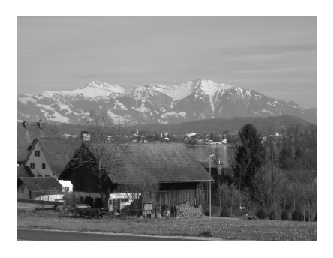
\includegraphics{obrazky/informatika/image_compression/image}
    }

    \subfigure[Obrázok magnitúdy koeficientov (použitá funkcia 
    $\log1+|x|$). Vľavo DFT, vpravo DCT.]{
    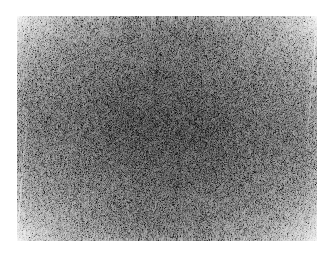
\includegraphics{obrazky/informatika/image_compression/dft}
    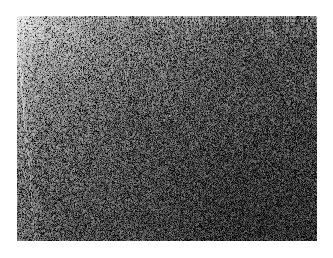
\includegraphics{obrazky/informatika/image_compression/dct}
    }
    \subfigure[Histogram pre magnitúdu. Vľavo DFT, v strede DCT a
    napravo porovnanie]{
    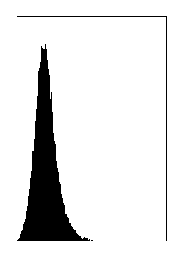
\includegraphics{obrazky/informatika/image_compression/dft_histogram}
    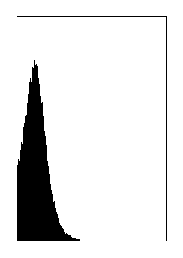
\includegraphics{obrazky/informatika/image_compression/dct_histogram}
    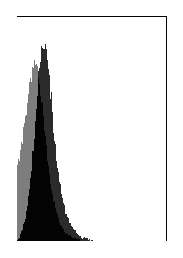
\includegraphics{obrazky/informatika/image_compression/combined_histogram}
    }
    \caption{Porovnanie koncentrácie energie pre DFT a DCT}
    \label{fig:dct_vs_dft}
\end{figure}
%% }}}


%\subsubsection{Jpeg kompresia }
\subsection{Jpeg kompresia }
Nasleduje posledná fáza a~tou je kompresia. Kompresia bude fungovať
rôzne pre DC člen (0,0) a~zvyšných 63 koeficientov. DC člen spravidla nesie 
v~sebe väčšinu energie a navyše je známe, že sa veľmi nemení medzi
susednými blokmi $8\cross8$, preto sa počíta ako rozdiel od predchádzajúceho
DC člena. AC koeficienty sa najskôr zoradia do cik-cak
postupnosti na obrázku \ref{fig:jpeg_zig_zag}. 

\begin{figure}[htp]
    \centering
    \includegraphics{obrazky/informatika/image_compression/zig_zag}
    \caption{JPEG formát - postupnosť v akej sú kódované AC koeficienty}
    \label{fig:jpeg_zig_zag}
\end{figure}

Zoradenie koeficientov
do tejto postupnosti je pomerne dôležité, pretože empiricky zoraďuje
najskôr najväčšie koeficienty a~potom tie menšie až nulové.
Finálna kompresia je tzv. "entropy coding". JPEG špecifikuje dva možné
prístupy - aritmetické kódovanie a~Huffmanovo kódovanie. Aritmetické
kódovanie produkuje o~5-10\% lepšie výsledky, avšak je náročnejšie 
a~pre rýchle implementácie JPEGu sa používa spravidla Huffmanov kód.
Samotné Huffmanovo kódovanie nebudeme rozoberať v~tejto publikácii,
po poznatkoch túžiaci čitateľ veľmi ľahko nájde literatúru na túto
tému.

%\subsubsection{Ďalšie aspekty JPEGu}
\subsection{Ďalšie aspekty JPEGu}

Existuje množstvo ďalších aspektov, ktoré sme v~tomto krátkom úvode
nespomenuli, a~stoja za zmienku. Existuje bezstratová verzia JPEGu,
ktorá funguje na úplne inom princípe. Navyše ukladanie dát je možné
rôznymi spôsobmi - sekvenčné a~progresívne ukladanie majú každé svoje
výhody. JPEG súbor ako taký môže tiež obsahovať náhľad obrázku, 
môže obsahovať viacero vrstiev.
Jednou z~otázok, ktoré mohli čitateľovi skrsnúť v~hlave je "Prečo
práve $8\cross8$?" Prečo sa neoplatí spraviť väčšie bloky? Výhodou malých
blokov je ich lokálnosť - veľké bloky majú väčšiu náchylnosť
kvantizáciou zmeniť obrazovú informáciu až príliš. Boli vyskúšané
bloky väčších veľkostí a~kvalita kompresie ostala porovnateľná.
Uvážením výpočtovej náročnosti kompresie a~dekompresie, bloky
veľkosti $8\cross8$ sa ukazujú ako veľmi dobrá voľba.

Viacej informácii o~tomto formáte sa čitateľ môže dočítať v
\cite{wiki:jfif}, \cite{wiki:jpeg} a~vynikajúcom popise JPEG kompresie
v \cite{wallace1991}.
